\documentclass[14pt, a4paper]{report}
\usepackage{mathtext}
\usepackage[T2A]{fontenc}
\usepackage[utf8]{inputenc}
\usepackage[russian]{babel}
\usepackage{multirow}
\usepackage{slashbox}
\usepackage{makecell}
\usepackage{graphicx}
\usepackage{physics}
\usepackage{amstext}
\usepackage{caption}
\usepackage{subcaption}

\renewcommand{\thesection}{\arabic{section}.}
\renewcommand{\thesubsection}{\arabic{section}.\arabic{subsection}.}

\title{\textbf{Отчет о выполнении лабораторной работы 2.2.3 "Измерение теплопроводности воздуха при атмосферном давлении"}}
\author{Калашников Михаил, Б03-205}
\date{}

\begin{document}
\maketitle

\textbf{Цель работы:}
измерить коэффициент теплопроводности воздуха при атмосферном давлении в зависимости от температуры.
\newline

\textbf{В работе используются:}
\begin{itemize}
\item цилиндрическая колба с натянутой по оси нитью ($2r_1=50\pm3\ мкм$, $2r_0=7,0\pm0,1\ мм$, $L=400\pm2\ мм$);
\item термостат ($\sigma_{t}=0,1\ ^\circ C$);
\item вольтметр ($\varepsilon_{U}=0,012\%$) и амперметр ($\varepsilon_{I}=0,05\%$) (цифровые мультиметры);
\item источник постоянного напряжения;
\item магазин сопротивлений ($0,1\ Ом$ -- $99999,9\ Ом$)
\end{itemize}

\section{Теоретические сведения}

Теплопроводность -- это процесс передачи тепловой энергии от нагретыхчас тей системы к холодным за счёт хаотического движения частиц среды. В газах теплопроводность осуществляется за счёт непосредственной передачи кинетической энергии от быстрых молекул к медленным при их столкновениях.
Перенос тепла описывается законом Фурье, утверждающим, что плотность потока энергии $\vec{q}$ пропорциональна градиенту температуры $\nabla T$
\[\vec{q}=\kappa\nabla T\]
где $\kappa$ -- коэффициент теплопроводности. Его можно пропопрционален квадратному корню из температуры:
\[\kappa\sim\lambda\bar{v}nc_V=\frac{1}{\sigma}\sqrt{\frac{8kT}{\pi m}}\frac{i}{2}R\propto\sqrt{T}\]

В случае, когда тепло выделяется в длинном проводе, размещенном в оси полого цилиндра той же длины и теплопроводность стационарна, нетрудно получить, что тепловая мощность провода равна
\[Q=\frac{2\pi L}{\ln r_0/r_1}\kappa\Delta T\]
где $r_1$ -- радиус провода, $r_0$ -- радиус цилиндра, $L$ -- длина провода, $\Delta T$ -- перепад температуры между проводом и стенками цилиндра.

\section{Экспериментальная установка}

Схема установки приведена на рис. 1. На оси полой цилиндрической трубки с внутренним диаметром $2r_0$ размещена металлическая нить диаметром $2r_1$ и длиной $L$. Полость трубки заполнена воздухом. Стенки трубки помещены в кожух, через которых пропускается вода из термостата, так что их температура $T_0$ поддерживается постоянной.

Для измерения напряжения и тока используется два мультиметра, работающие в режимах вольтметра и амперметра соответственно. Подключение к нити $R_н$ осуществляется по четырёхпроводной схеме. По двум проводам через сопротивление пропускается измерительный ток, а два других используются для параллельного подключения вольтметра.

\begin{figure}
\centering
\begin{subfigure}{.4\textwidth}
 \centering
 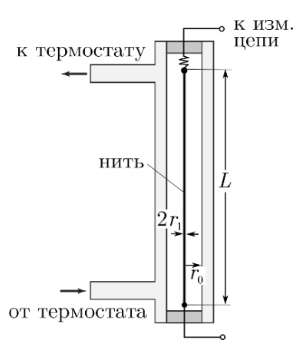
\includegraphics[width=1\linewidth]{terma6_00.png}
\end{subfigure}%
\begin{subfigure}{.4\textwidth}
\centering
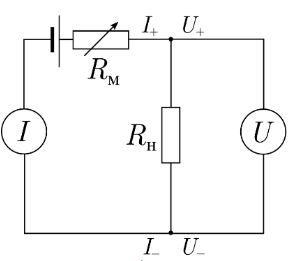
\includegraphics[width=1\linewidth]{terma6_01.png}
\end{subfigure}
\caption{Схемы установки и цепи}
\end{figure}

\section{Проведение эксперимента}

\begin{enumerate}

\item Предварительно рассчитаем максимальные допустимые значения напряжения $U_{макс}$ и $I_{макс}$ тока на нити из формулы
\[Q=\frac{2\pi L}{\ln r_0/r_1}\kappa\Delta T\]
используя приближенные значения параметров установки. Получим:
\[U_{макс}=2,7\ В\quad I_{макс}=130\ мА\]

\item Выставим максимальное значение сопротивления на магазине сопротивлений. Включим вольтметр и амперметр, настроим их на нужный режим работы. Запустим источник питания и термостат.

\item Выставим на термостате комнатную температуру и будем фиксировать показания приборов, постепенно уменьшая сопротивление магазина $R_м$. Занесем данные в таблицу 2.
Значения сопротивления $R_м$ были предварительно рассчитаны таким образом, чтобы мощность, выделяемая проволокой, возрастала монотонно в диапазоне от $0$ до $Q_{макс}$ (таблица 1).

\item Вновь выставим на магазине максимальное сопротивление.

\item Повторим предыдущие два пункта еще шесть раз постепенно увеличивая температуру термостата и дожидаясь ее установления.

\item Выключим все измерительные приборы, блок питания, на магазине сопротивлений установим максимальное сопротивление, а на термостате установим комнатную температуру.

\end{enumerate}

\section{Обработка данных}

\begin{enumerate}

\setcounter{enumi}{6}

\item Для каждой температуры построим зависимость $R(Q)$ ($R=\frac{U}{I},\ Q=UI$). Через точки проведем прямую МНК. Рассчитаем значения $R_0=R(0)$ и $\dv{R}{Q}$ и занесем их в таблицу 3.

\item Через точки $R_0$, полученные в предыдущем пункте, построим прямую МНК. Заметим, что на прямую ложатся только первые три точки, поэтому в дальнейшем будем использовать только их. Получим зависимость $R(T)$. Рассчитаем температурный коэффициент сопротивления нити $\alpha$ по формуле:
\[\alpha=\frac{1}{R(T_0)}\dv{R}{T},\quad T_0=273\ К\]

\item Используя результаты предыдущих пунктов, вычислим наклон зависимости выделяющейся на нити мощности $Q$ от ее перегрева $\Delta T$ относительно стенок:
\[\dv{Q}{\Delta T}=\dv{R}{T}/\dv{R}{Q}\]
Дополним таблицу 2.

\item Зная, что $\dv{Q}{\Delta T}=\frac{2\pi L}{\ln r_0/r_1}\kappa$, вычислим значение коэффициента теплопроводности $\kappa$:
\[\kappa=\frac{\ln r_0/r_1}{2\pi L}\dv{Q}{\Delta T}\]
Результаты также занесем в таблицу.

\item Построим график зависимости $\kappa(T)$ в двойной логарифмическом масштабе и определим показатель степени в зависимости $\kappa\propto T^\beta$.

\end{enumerate}

\section{Расчет погрешностей}

Определим относительную погрешность величин, полученных в пункте 7. Пусть зависимость $R(Q)$ имеет вид $R=kQ+b$. Тогда:
\[\varepsilon_{\dv{R}{Q}}=\sqrt{\varepsilon_{k}^2+\varepsilon_{U}^2+\varepsilon_{I}^2}=0,9\%\]
\[\varepsilon_{R_0}=\sqrt{\varepsilon_{b}^2+\varepsilon_{U}^2+\varepsilon_{I}^2}=0,08\%\]

Определим погрешность $\dv{R}{T}$ из МНК:
\[\varepsilon_{\dv{R}{T}}=\sqrt{\varepsilon_{k}^2+\varepsilon_{R_0}^2+\varepsilon_{t}^2}=2,0\%\]

Величина $1/\varepsilon_{\dv{R}{T}}\approx50$ удовлетворяет критерию Стьюдента при $n-k-1=1$ и $p=0,95$, равному 12,7.

Погрешность величины $\alpha$ выражается по формуле:
\[\varepsilon_{\alpha}=\sqrt{\frac{\sigma_k^2 T_0^2+\sigma_b^2}{(kT_0+b)^2}+\varepsilon_{\dv{R}{T}}^2}=2,0\%\]
\[\alpha=0,49\pm0,01\ \frac{10^{-3}}{К}\]

Найдем погрешность $\dv{Q}{\Delta T}$:
\[\varepsilon_{\dv{Q}{\Delta T}}=\sqrt{\varepsilon_{\dv{R}{Q}}^2 + \varepsilon_{\dv{R}{T}}^2}=2,2\%\]

Вычислим погрешность коэффициента теплопроводности:
\[\varepsilon_{\kappa}=\sqrt{\frac{\varepsilon_{r_0}^2+\varepsilon_{r_1}^2}{\ln^2(r_0/r_1)}+\varepsilon_{L}^2+\varepsilon_{\dv{Q}{\Delta T}}^2}=2,6\%\]

Наконец, определим погрешность коэффициента $\beta$:
\[\frac{\sigma_{\beta}}{\beta}=\frac{1}{\beta}\sqrt{\varepsilon_{\kappa}^2+\varepsilon_{t}^2+\sigma_{k}^2}=13\%\]
\[\beta=0.42\pm0.06\]

\section{Вывод}

В результате работы, несмотря на осложнения, вызванные данными, полученными при высоких температурах термостата, получилось определить коэффициент $\beta$, приближенный к его действительному значению, равному $0,5$. Температурный коэффициент сопротивления платины $\alpha$, однако, сильно отличнается от настоящего значения, равного $=3,9\cdot10^{-3}\ \frac{1}{К}$.

\section{Приложения}

\begin{table}[!ht]
\centering
\makebox[\textwidth][c] {
\begin{tabular}{| c | c | c | c | c | c | c | c | c | c | c | c |}
\hline
$\eta$ & 0,01 & 0,1 & 0,2 & 0,3 & 0,4 & 0,5 & 0,6 & 0,7 & 0,8 & 0,9 & 1 \\
\hline
$R_м,\ Ом$ & 180 & 43,2 & 24,7 & 16,5 & 11,6 & 8,3 & 5,8 & 3,9 & 2,4 & 1,1 & 0 \\
\hline
\end{tabular}
}
\caption{Значения $R_м$, подобранные для монотонного возрастания мощности, выделяемой нитью ($Q=\eta\cdot Q_{макс}$)}
\end{table}

\begin{table}[!ht]
\centering
\makebox[\textwidth][c] {
\begin{tabular}{| c | c | c | c | c | c | c | c | c | c | c | c | c |}
\hline
$t,\ ^\circ C$ & $\eta$ & 0,01 & 0,1 & 0,2 & 0,3 & 0,4 & 0,5 & 0,6 & 0,7 & 0,8 & 0,9 & 1 \\
\hline
\multirow{2}{*}{27,9}	& $I,\ мА$	& 16,596	& 48,935	& 66,188	& 78,235	& 87,671	& 95,289	& 101,92	& 107,55	& 112,36	& 116,81	& 142,48 \\
				& $U,\ В$ 	& 0,3461	& 1,0326	& 1,4123	& 1,6857	& 1,9055	& 2,0872	& 02,249	& 02,389	& 02,511	& 2,6252	& 3,3196 \\
\hline
\multirow{2}{*}{35,0}	& $I,\ мА$	& 16,556	& 48,879	& 66,099	& 78,121	& 87,537	& 95,137	& 101,76	& 107,37	& 112,16	& 116,60	& 142,20 \\
				& $U,\ В$	& 0,3465	& 1,0349	& 1,4147	& 1,6879	& 1,9075	& 2,0889	& 2,2504	& 02,390	& 2,5117	& 2,6262	& 3,3191 \\
\hline
\multirow{2}{*}{40,0}	& $I,\ мА$	& 16,549	& 48,836	& 66,013	& 78,020	& 87,403	& 97,523	& 101,58	& 107,19	& 111,97	& 116,41	& 141,95 \\
				& $U,\ В$	& 0,3472	& 1,0364	& 1,4163	& 1,6894	& 1,9089	& 2,1518	& 2,2512	& 2,3910	& 02,512	& 2,6265	& 3,3183 \\
\hline
\multirow{2}{*}{45,0}	& $I,\ мА$	& 16,681	& 48,827	& 66,010	& 78,002	& 87,397	& 94,983	& 101,59	& 107,21	& 112,00	& 116,45	& 141,99 \\
				& $U,\ В$	& 0,3483	& 1,0374	& 1,4174	& 1,6906	& 1,9101	& 2,0916	& 2,2528	& 2,3926	& 2,5138	& 2,6282	& 3,3203 \\
\hline
\multirow{2}{*}{50,0}	& $I,\ мА$	& 16,591	& 48,861	& 66,055	& 78,056	& 87,745	& 95,045	& 101,65	& 107,28	& 112,07	& 116,52	& 142,09 \\
				& $U,\ В$	& 0,3483	& 1,0376	& 1,4177	& 1,6910	& 1,9106	& 2,0920	& 2,2532	& 2,3931	& 02,514	& 2,6288	& 3,3213 \\
\hline
\multirow{2}{*}{55,1}	& $I,\ мА$	& 16,593	& 48,872	& 66,078	& 78,088	& 87,494	& 95,092	& 101,70	& 107,33	& 112,13	& 116,59	& 142,18 \\
				& $U,\ В$	& 0,3481	& 1,0372	& 1,4173	& 1,6906	& 1,9102	& 2,0917	& 2,2529	& 2,3927	& 2,5141	& 2,6285	& 3,3214 \\
\hline
\multirow{2}{*}{60,1}	& $I,\ мА$	& 16,594	& 48,887	& 66,103	& 78,123	& 87,539	& 95,143	& 101,76	& 107,40	& 112,20	& 116,65	& 142,27 \\
				& $U,\ В$	& 0,3478	& 1,0363	& 1,4163	& 1,6896	& 1,9093	& 2,0908	& 2,2522	& 2,3921	& 2,5134	& 2,6280	& 3,3215 \\
\hline
\end{tabular}
}
\caption{Данные, полученные в ходе выполнения работы}
\end{table}

\begin{table}[!ht]
\centering
\makebox[\textwidth][c] {
\begin{tabular}{| c | c | c | c | c | c | c | c |}
\hline
$t,\ ^\circ C$ & 27,9 & 35,0 & 40,0 & 45,0 & 50,0 & 55,1 & 60,1 \\
\hline
$R_0,\ Ом$ & 20,85 & 20,92 & 20,97 & 20,96 & 20,97 & 20,97 & 20,95 \\
$\dv{R}{Q},\ Ом/Дж$ & 5,26 & 5,20 & 5,17 & 5,26 & 5,14 & 5,12 & 5,13 \\
$\dv{Q}{\Delta T},\ мДж/К$ & 1,92 & 1,94 & 1,95 & - & - & - & - \\
$\kappa,\ мкВт/(м\cdot К)$ & 3,8 & 3,8 & 3,8 & - & - & - & - \\
\hline
\end{tabular}
}
\caption{Значения $R_0$ и $\dv{R}{Q}$ для различных температур}
\end{table}


\begin{figure}[!ht]
\centering
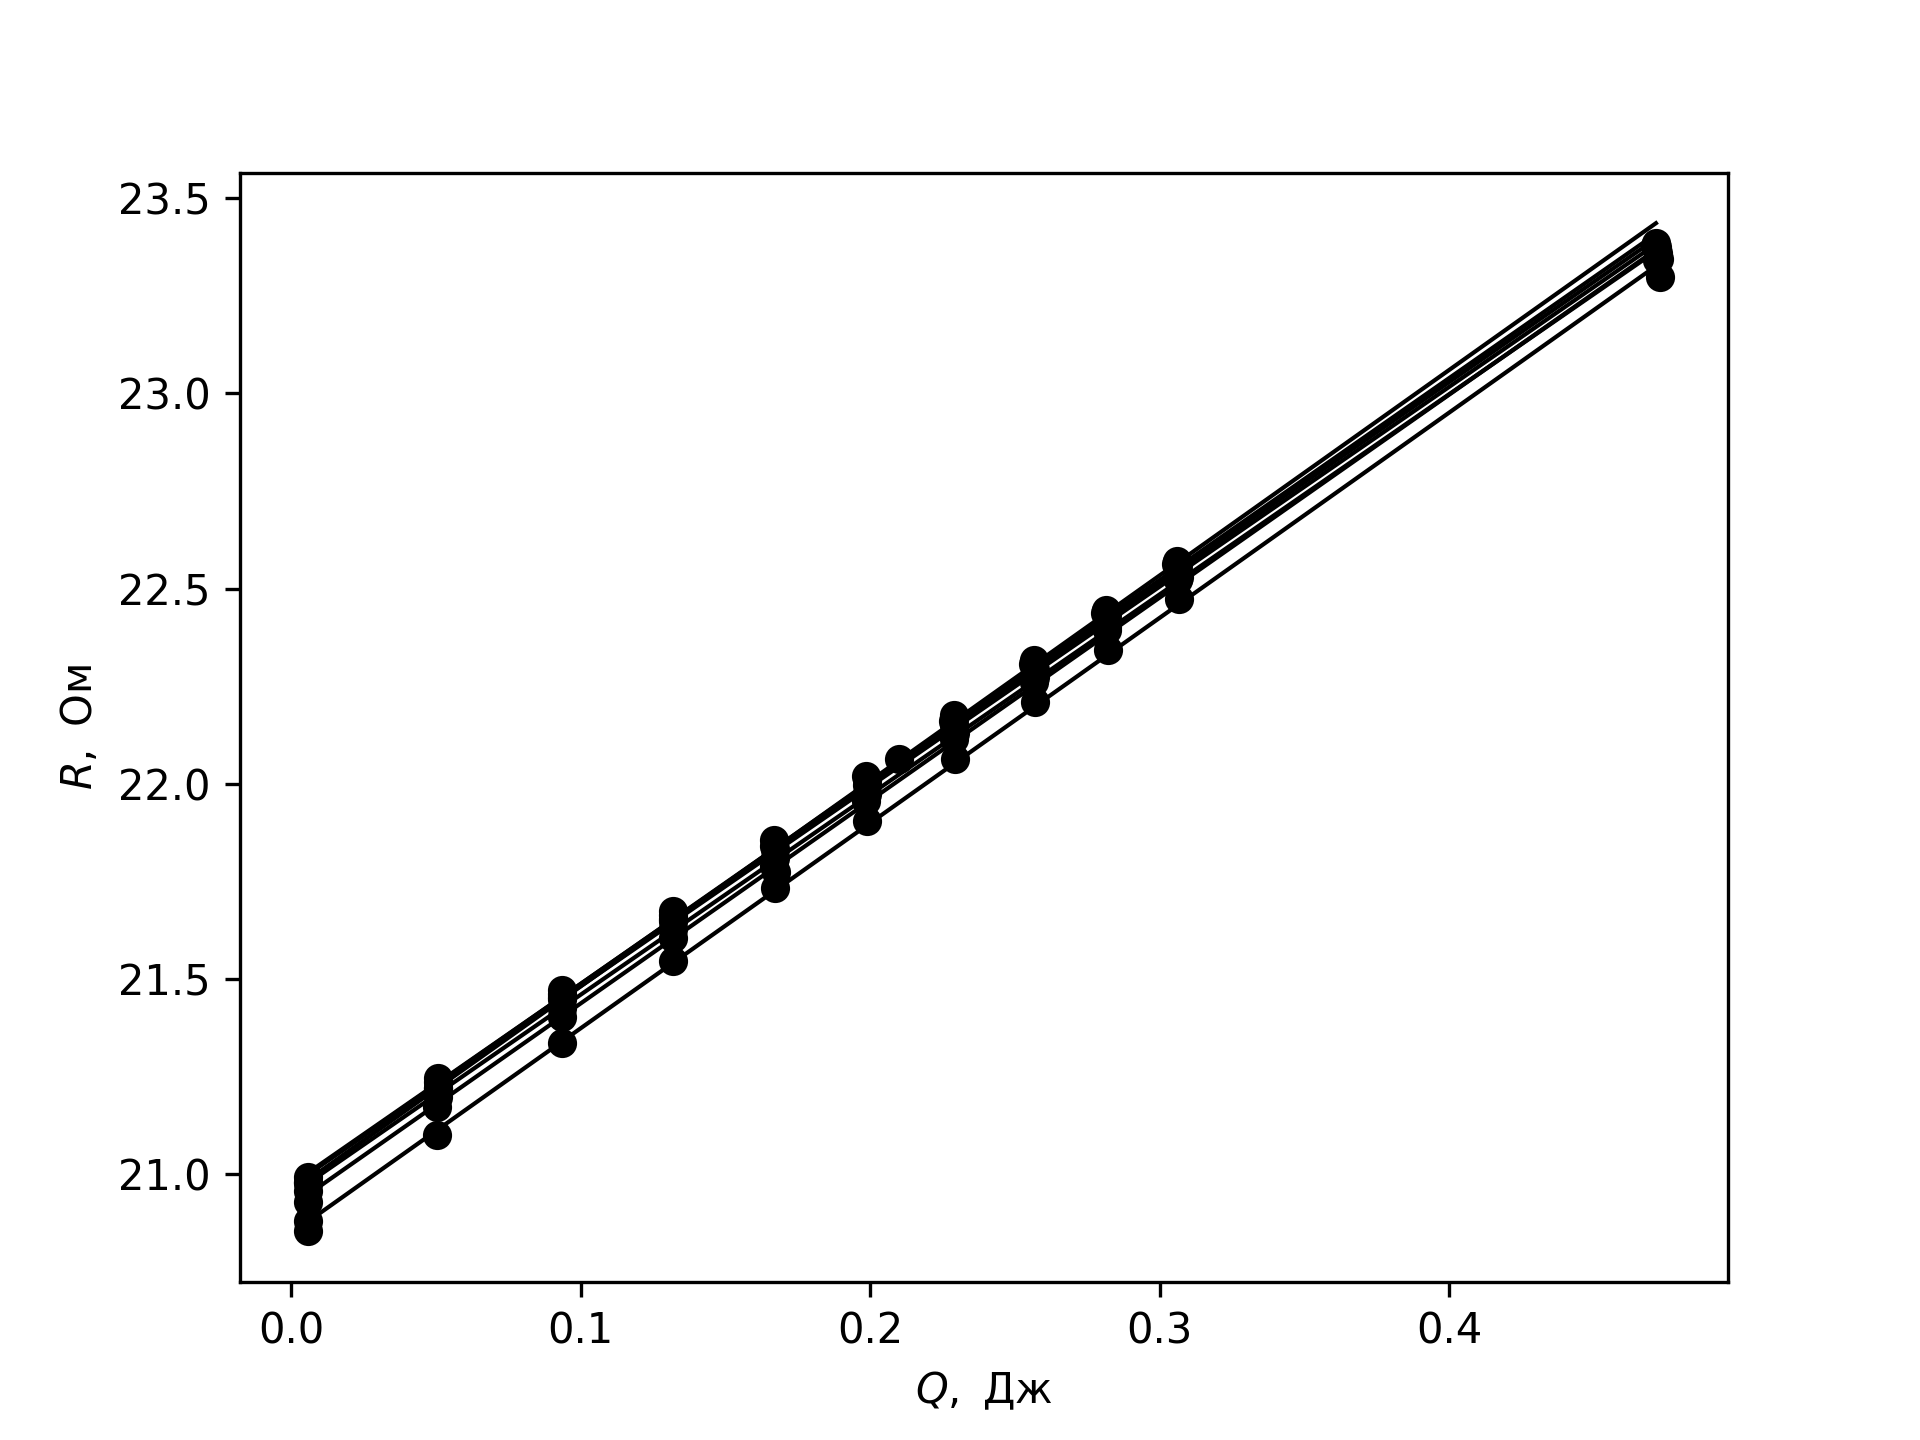
\includegraphics[scale=0.6]{terma6_1.png}
\caption{Графики зависимостей $R(Q)$ для различных температур}
\end{figure}


\begin{figure}[!ht]
\centering
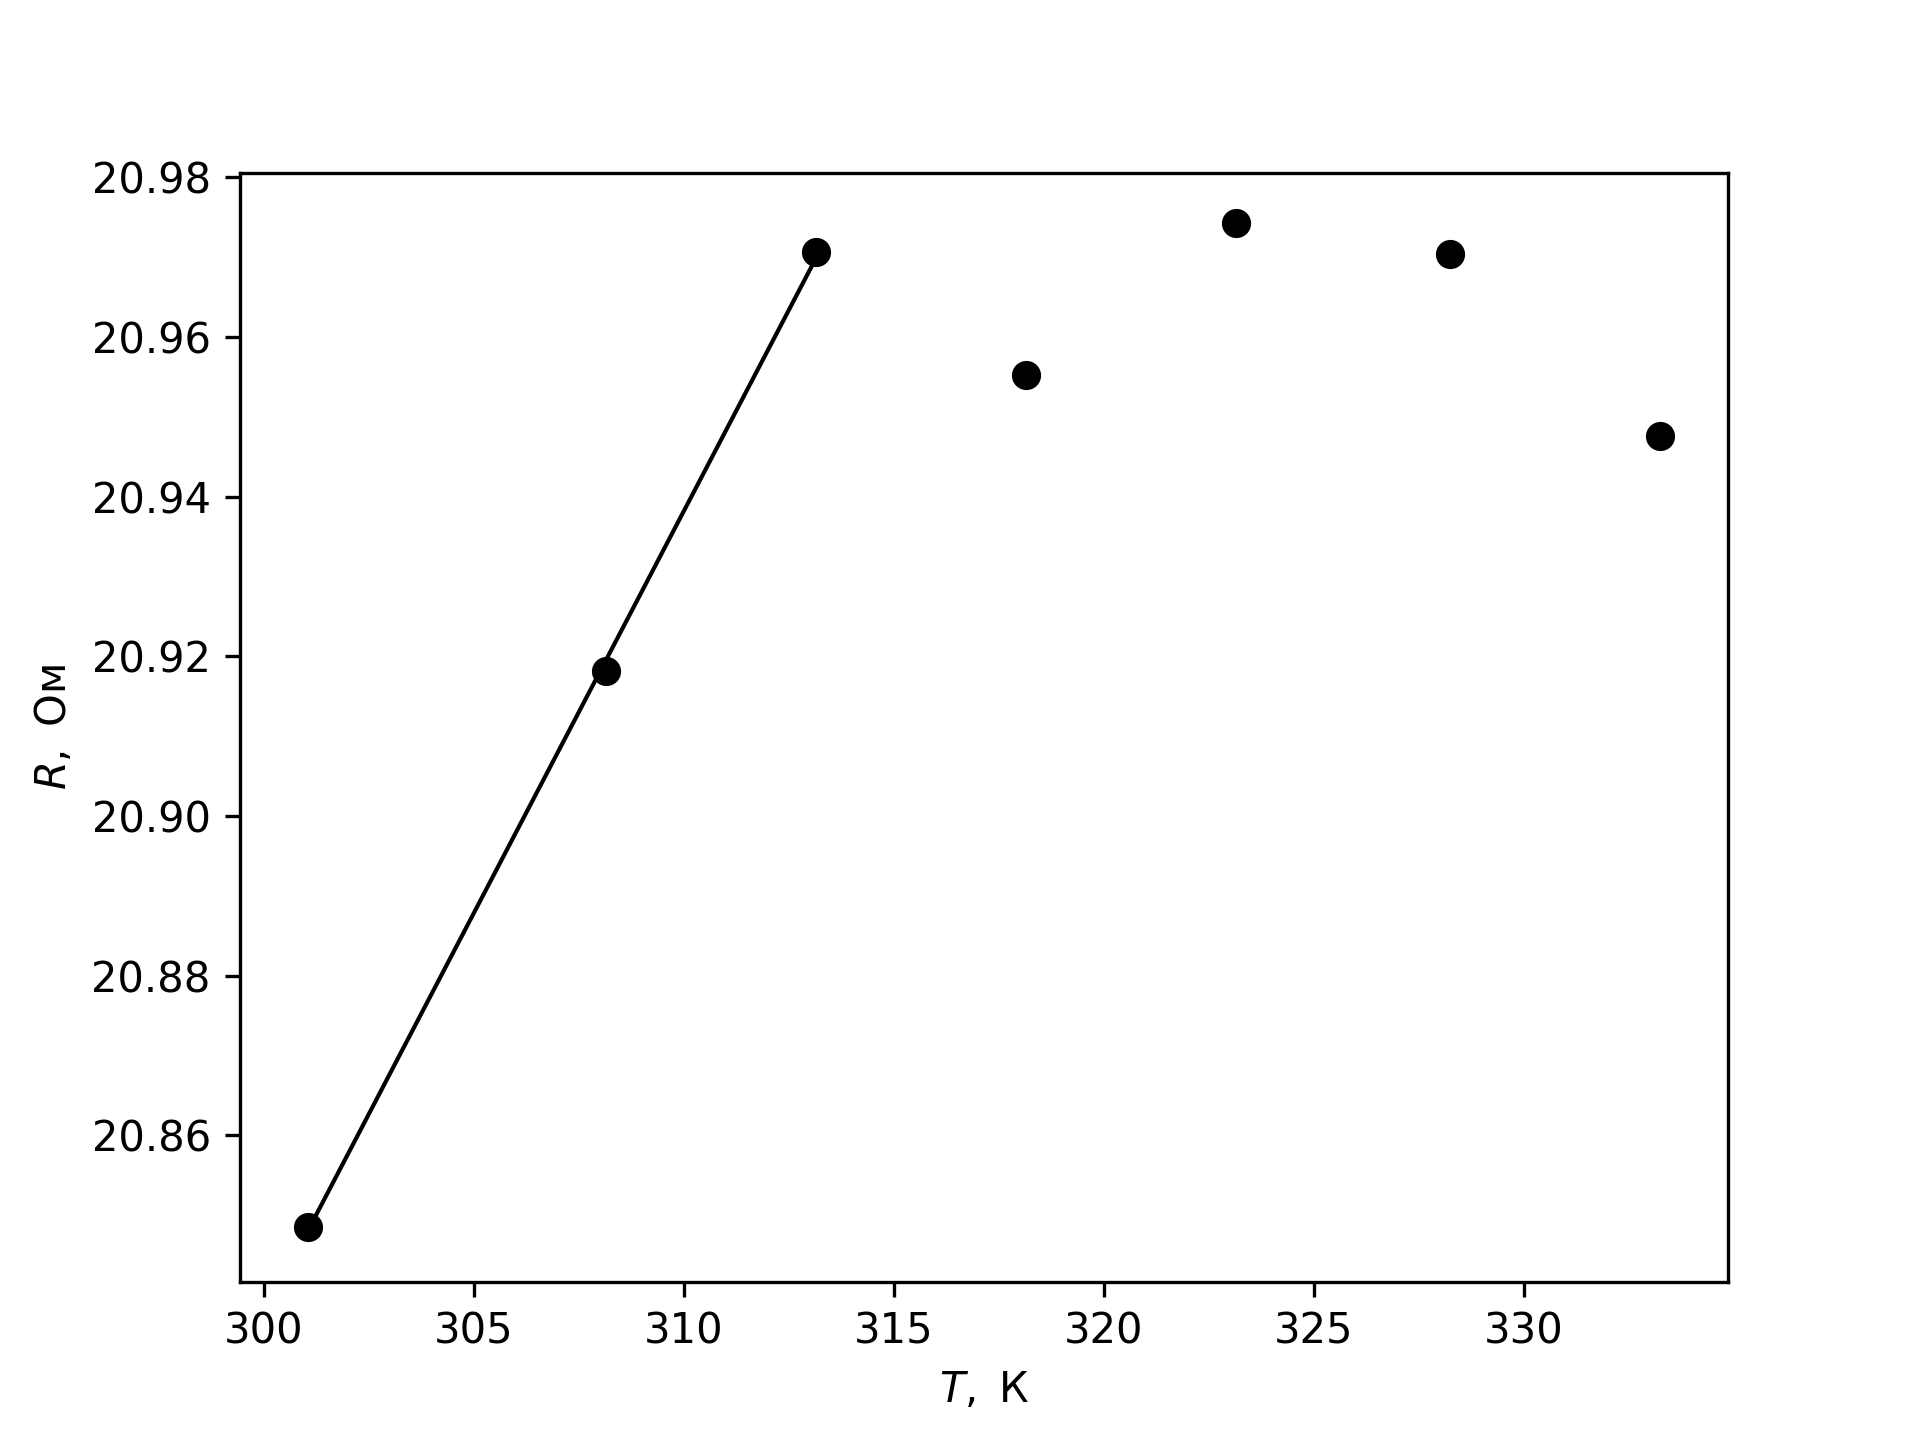
\includegraphics[scale=0.6]{terma6_2.png}
\caption{Графики зависимости $R(T)$}
\end{figure}

\begin{figure}[!ht]
\centering
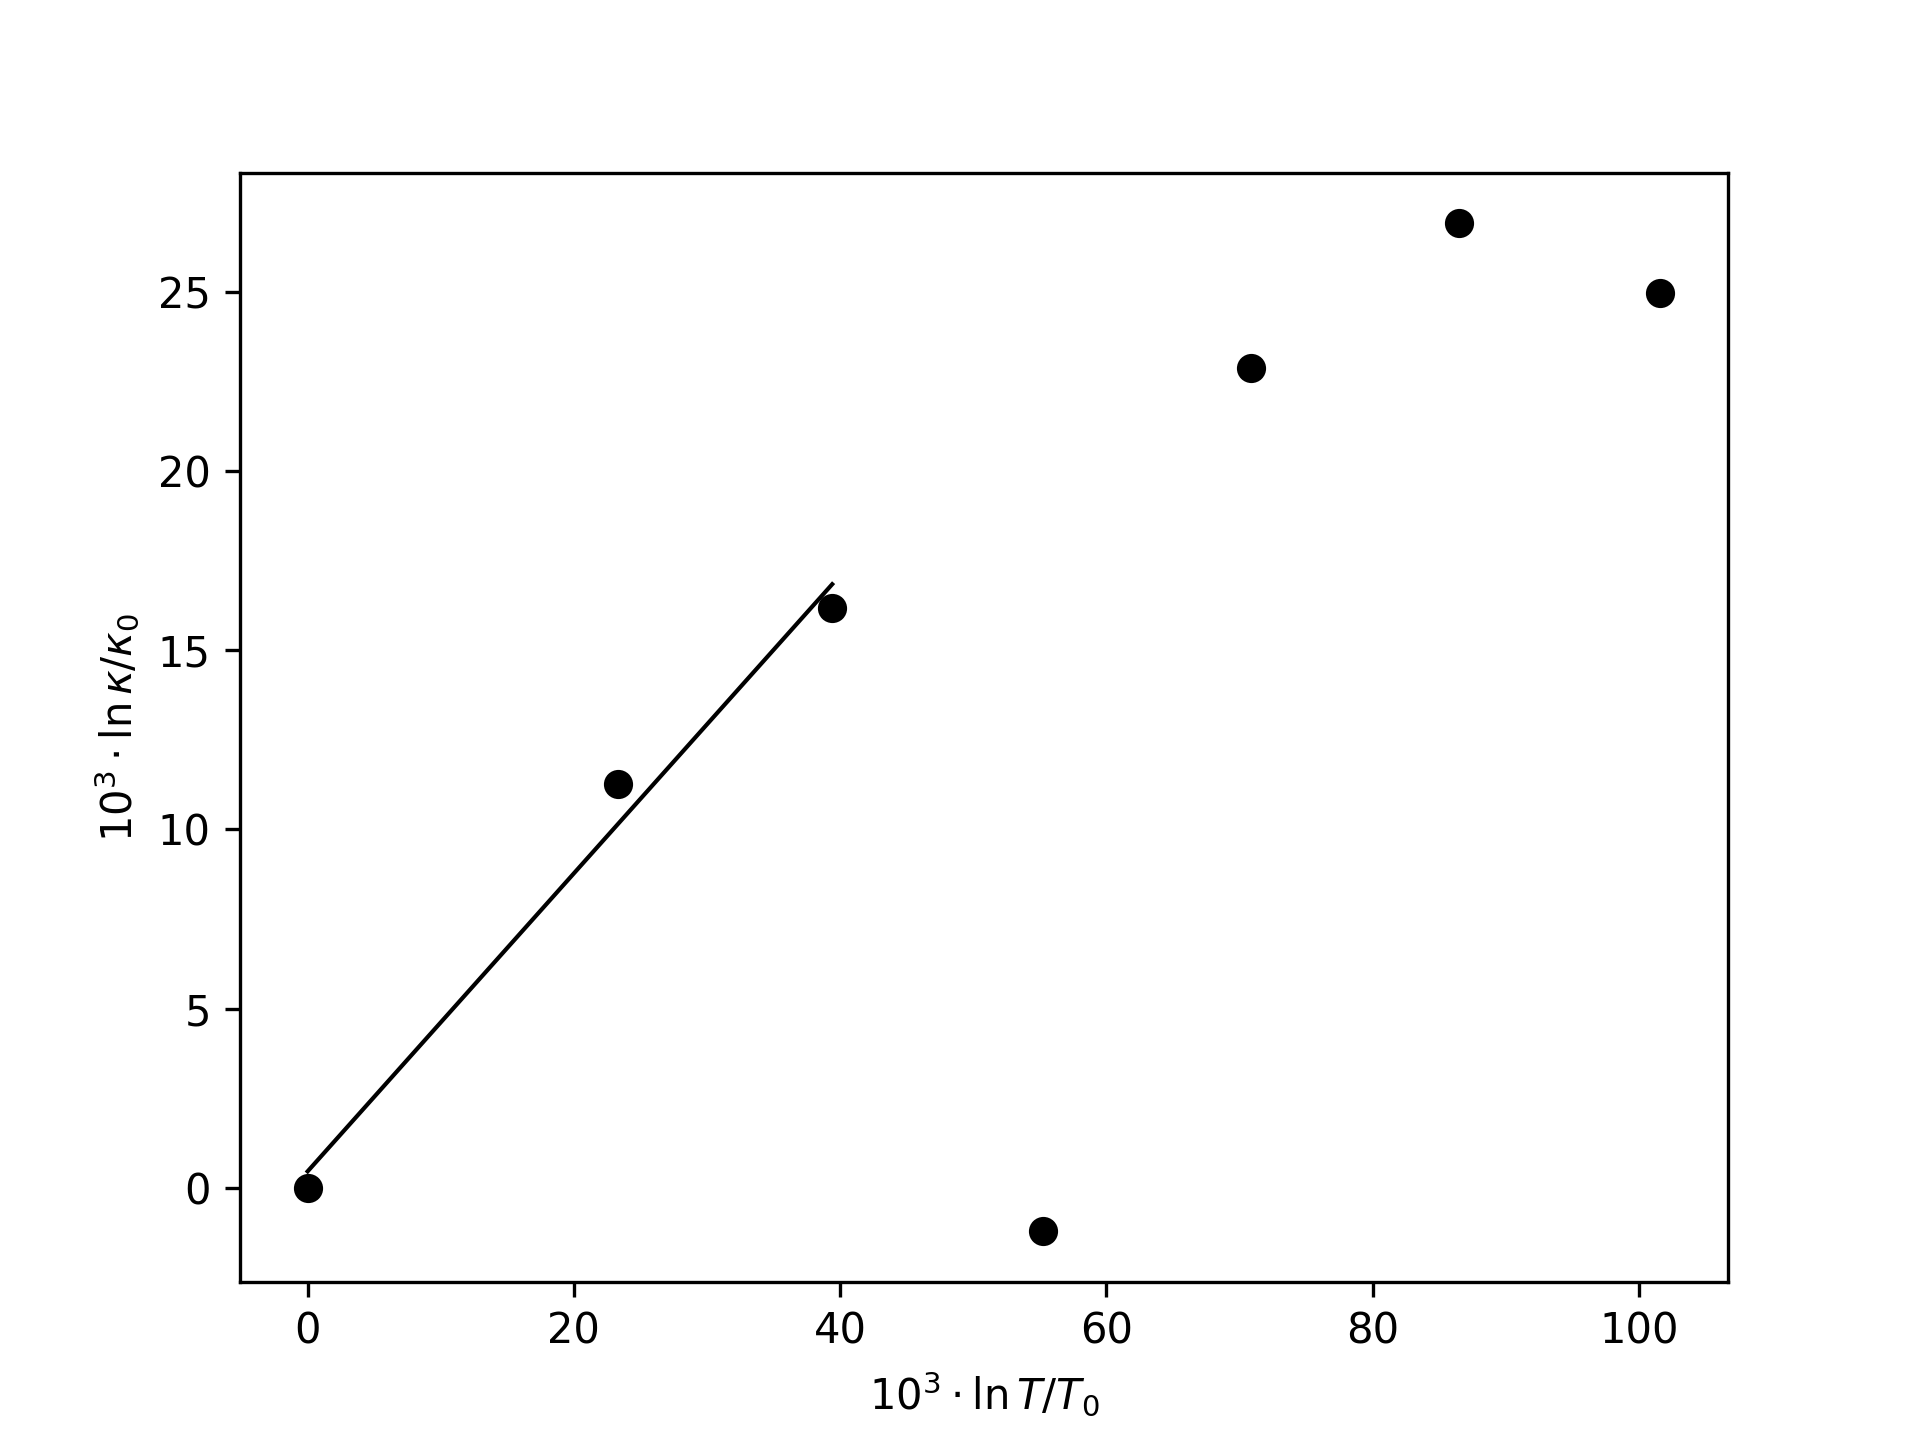
\includegraphics[scale=0.6]{terma6_3.png}
\caption{Графики зависимости $\ln\kappa(\ln T)$, отнормированный таким образом, что первая точка совпадает с точкой $(0, 0)$}
\end{figure}

\end{document}